\subsection{Alternative to $\hat{\textbf{A}}$}  
As concluded the COV-DL algorithm do not recover a sufficient mixing matrix $\mathbf{A}$ and therefore other actions must be taken. 

Instead a fixed mixing matrix $\mathbf{A}_{\text{fixed}}$ could be a better choice. However, this fixed mixing matrix must have some of the same characteristic as the true mixing matrix. 
From observations of the true mixing matrix from the autoregressive data set some choice could be:
\begin{itemize}
\item A matrix drawn from uniform distribution in the half open interval $[-1.0, 1.0)$.
\item A matrix drawn from random distribution with mean $0$ and variance $2$.
\item A matrix drawn from a Gaussian distribution with mean $0$ and variance $1$.
\item A matrix computed from ICA of EEG measurements provided from EEGLab\footnote{EEGLab is an interactive Matlab toolbox for processing EEG measurements.}.
\end{itemize}
The test of the different mixing matrices $\mathbf{A}_{\text{fixed}}$ is performed in the autoregressive data set specified for $M = 8$, $k = 8$ and $L = 1000$. Each test of one mixing matrix will be run ten times resulting in an average MSE value. For this test both MSE value for the source matrix $\mathbf{X}$ and the fixed mixing matrix compared to the true mixing matrix will be calculated. 
The MSE of the four fixed mixing matrices can be seen in table \ref{tab:fixed}.
\begin{table}[H]
\centering
\begin{tabular}{|c|c|c|c|c|}
\hline
 & Uniform & Random & Gaussian & EEG \\
\hline
MSE$_\mathbf{A}$ & 1.26 & 4.65 & 2.08 & 1.16 \\
\hline
MSE$_\mathbf{X}$ & 22.93 & 8.30 & 12.95 & 103.76 \\
\hline
\end{tabular}
\caption{MSE values from measurement specified by $M=8$, $k=16$ and $L=1000$ with a fixed mixing matrix $\mathbf{A}_{\text{fixed}}$.}
\label{tab:fixed}
\end{table}
\noindent
The argument behind which mixing matrix will be the best fit was to take the one with the lowest MSE as this must also lead to a low error for the source matrix. As seen in table \ref{tab:fixed} this is not the case as the lowest MSE for the mixing matrix is with the EEG mixing matrix but this lead to the highest MSE for the source matrix. 
The choice must then be based on where the two error intersect with each other.
\begin{figure}[H]
\centering
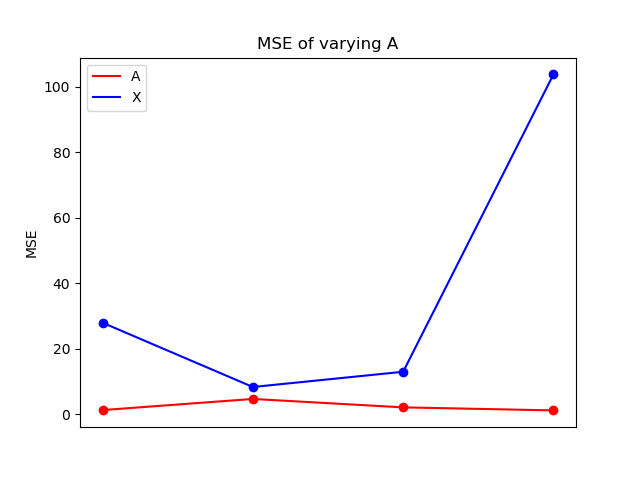
\includegraphics[scale=0.5]{figures/ch_6/AR_Error_vary_A_m8_k16_N16_L1000.png}
\caption{MSE values for the mixing matrix and the source matrix with fixed mixing matrix.}
\end{figure}
\noindent
From table \ref{tab:fixed} and the figure it seen that the mixing matrix drawn from the random distribution lead to the MSE values being close to each other and to the lowest MSE value of the source matrix. As the main interest in this thesis is to identify and localise the active sources of EEG measurement a low MSE of the source matrix may seem more desirable than a low MSE value for the mixing matrix. 

From these observation a mixing matrix drawn from a random distribution with mean 0 and variance 2 lead to a suitable MSE of both the mixing matrix and source matrix and will then be the choice of a fixed mixing matrix when testing the baseline algorithm on real EEG measurements.
